\documentclass{jarticle}

% Language setting
% Replace `english' with e.g. `spanish' to change the document language
% \usepackage[english]{babel}
\usepackage[dvipdfmx]{graphicx}
\usepackage[dvipdfmx]{color}

% Set page size and margins
% Replace `letterpaper' with `a4paper' for UK/EU standard size
\usepackage[letterpaper,top=2cm,bottom=2cm,left=2cm,right=2cm,marginparwidth=1.75cm]{geometry}
% \usepackage[letterpaper,top=1cm,bottom=1cm,left=1cm,right=1cm,marginparwidth=1cm]{geometry}

% Useful packages
\usepackage{amsmath}
\usepackage{graphicx}
\usepackage[colorlinks=true, allcolors=blue]{hyperref}
\usepackage{longtable}
\usepackage{amsmath}
\usepackage{booktabs}
\usepackage{breqn}
\usepackage{lscape}
\usepackage{amsmath,amsthm,amssymb,multirow} %カンマで区切ることで一度にusepackageできる
%\usepackage{natbib}
\usepackage{here}
\usepackage{color}
\usepackage{bm}
%\usepackage{subfig}
\usepackage{subcaption}
\usepackage{listings, jlisting}
\usepackage{txfonts}
\usepackage{comment}
\usepackage{ascmac}
\usepackage{algorithm}
\usepackage{algorithmic}
\usepackage{tabularx}

% \usepackage{fancybx}
\newcommand{\mathbm}[1]{{\mbox{\boldmath $#1$}}}
\newcommand{\rd}{\partial}
\newcommand{\dd}[2]{\dfrac{\partial #1}{\partial #2}}
\newcommand{\ddd}[2]{\dfrac{\partial^2 #1}{\partial #2^2}}
\newcommand{\dddd}[3]{\dfrac{\partial^2 #1}{\partial #2 \partial #3}}
\newcommand{\ol}{\overline}
\newcommand{\bibname}{参考文献}
\renewcommand{\figurename}{図}
\renewcommand{\tablename}{表}
\renewcommand{\lstlistingname}{ソースコード}
\newcommand{\keywords}[1]{\par\noindent{\small\textbf{キーワード:} #1}\par\vspace{1em}}
\newcommand{\Eqref}[1]{式~(\ref{#1})}
\newcommand{\Figref}[1]{図~\ref{#1}}
\newcommand{\Tblref}[1]{表~\ref{#1}}
\newcommand{\Coderef}[1]{ソースコード~\ref{#1}}
\newcommand{\Algref}[1]{Algorithm~\ref{#1}}
\newcommand{\red}[1]{\textcolor{red}{#1}}
\newcommand{\blue}[1]{\textcolor{blue}{#1}}
% \newcommand{\yellow}[1]{\textcolor{yellow}{#1}}
% \newcommand{\violet}[1]{\textcolor{violet}{#1}}

\theoremstyle{plain}
\newtheorem{thm}{Theorem}
\newtheorem*{thm*}{Theorem}
\theoremstyle{definition}
\newtheorem{dfn}{Definition}

\title{LaTeXサンプル論文}
\author{サンプル著者}
\date{\today}

\begin{document}
\maketitle

\abstract{%
本論文では,SE(3)上における協調自己位置推定のための視野共有を保証する分散型制御バリア関数(CBF)手法を提案する.
マルチエージェントシステムにおいて,各エージェントが共通の視野を維持することは,特徴点マッチングによる協調自己位置推定の精度向上に不可欠である.
提案手法では,単一特徴点および複数特徴点の追従に対する安全制約を定式化し,確率的CBFを用いて視野共有を保証する.
さらに,非ホロノミックなドローンダイナミクスに対応するため,高次制御バリア関数(HOCBF)を導入し,SE(3)上の離散ダイナミクスを考慮した制約付き最適化問題を定式化する.
また,プライマル・デュアル乗数法(PDMM)を用いた分散実装により,中央集権的な制御なしでも視野共有を実現する手法を示す.
シミュレーション結果から,提案手法の有効性と分散実装の性能を検証する.
}

% \keywords{%
% 制御バリア関数,共有視野,SE(3),分散制御,マルチエージェントシステム,協調自己位置推定
% }

\section{序論}

\subsection{共有視野保証の重要性と背景}

マルチロボットシステムでは,各ロボットがセンサ情報や視界を共有することにより,監視・捜索・協調輸送などのタスクを効率的に遂行できることが知られている.
特にカメラを用いた視覚協調の場合,各ロボットの共有視野(Common Field-of-View, CoFoV)が不可欠である.例えば,複数ドローンが異なる角度から同一対象を観測できることや,通信の見通し線(LOS)維持が求められる\cite{Panagou2017}.

マルチエージェントVSLAM(Visual Simultaneous Localization and Mapping)においては,各エージェントが撮影した画像から抽出される局所特徴に基づき自己局在を行い,エージェント間で特徴マッチングにより相対位置を推定する.従来のORBやSIFTに代わり,SuperPointのような学習型局所特徴検出・記述器\cite{DeTone2018}や,NetVLADによるグローバル記述子\cite{Arandjelovic2016}が高いロバスト性を示し,ループ検出やキーフレームマッチングに貢献している.

画像特徴量のマッチングを成功させるためには,各エージェントが共通のランドマークを観測できるよう,カメラの視野錐台の幾何学的重複が必要である.視野重複が存在すれば,エージェント間でのループ検出が可能となり,その結果として各ロボットの地図統合が実現される\cite{Zhang2022}.しかし,ロボットは視野角が限られているため,視界共有を保証するための制御技術の開発が急務である.

\red{モチベーション:CoVINSではsuperpoint特徴量などの画像特徴量のマッチングにより、自己位置推定に関する最適化問題のfactorを得ている。特徴量をマッチングするにはエージェントの視野錐台が重なっている必要がある。single agent問題に関してはstereo cameraの相対位置をconstかつgivenとして最適化問題に組み込み、multi agent問題に関しては視野錐台のoverrideは不可知であるために画像全体特徴量の類似度の一致などによってpassiveなevent trigger型としてアルゴリズムが構築されている。しかし、agent1とagent2が視野錐台を交差させ続けるための制御則(CBF等)に基づいてactive perceptionを行う場合、multi agentの自己位置推定においてinter-agentな特徴量のマッチング及び推定問題はエージェントをまたいだカメラ間の相対位置をgiven, もしくは最適化すべき双対変数として複数のエージェント位置を同時最適化できるはずである。さらに、active perceptionの枠組みで考えれば、CBFを用いた最適制御問題と自己位置推定問題も同一の目的関数の最小化問題として扱うことができるはずである。  
上記の仮定から、本セミナーではその手始めとして,代表的なCoVINSであるUAVを対象として、視野錐台を交差させ続けるための分散型CBF手法を提案する。}

\subsection{既存研究の課題}

従来はポテンシャル場やMPC(Model Predictive Control)を用いた手法が提案され,局所的な視界制約下での隊列制御やセンサグラフの連結性維持に取り組まれてきた\cite{Sabattini2013}.一方で,制御バリア関数(Control Barrier Function, CBF)を用いた手法は,制約違反を防ぎながらリアルタイムに最適な制御入力を計算できるため,有力な候補となる\cite{Capelli2020}.

しかし,現状の協調SLAMは,キーフレームの受動的な共有と画像類似度評価に依存しており,視野重複が偶発的に発生しなければマップ統合が成立しないリスクがある.また,多数のロボットを対象とする場合,中央集権的な制御は通信負荷や計算量の面で現実的ではなく,各エージェントが局所的に計算し,限定的な通信で連携する分散アルゴリズムの設計が必要である.

従来の視野維持手法は,対象が視野内にあるか否かを決定論的に評価するに留まっていたが,センサの観測不確実性を十分に取り入れていなかった\cite{Panagou2012}.また,従来の多くの視野制約付き制御手法は,単純な動力学モデル(例:Dubins車両やクアッドロータの水平姿勢維持)に基づいており,非ホロノミックなダイナミクスを明示的に考慮していなかった\cite{Dias2016}.

\subsection{本研究の貢献}

本研究では,SE(3)上における協調自己位置推定のための視野共有を保証する分散型CBF手法を提案する.本研究の主な貢献は以下の通りである.

\begin{itemize}
\item SE(3)における共有視野保証を実現する.従来のステレオ視やリーダーフォロワ形式による視野制御は,ロボット間の相対配置を幾何学的に制約するに留まっていたが,本手法は3次元空間におけるエージェント全体の姿勢・位置を統合的に制御する枠組みを提供する.

\item 特徴点に基づく確率的可視性制約とCBFの適用を行う.本研究では,各エージェントが観測する特徴点に基づき,その可視性を確率的に評価した上で,CBFに組み込み,常時高い確率で共有視野が確保されるよう制御入力を設計する.これにより,センサノイズ等による不確実性下でも安全な視野維持が可能となる.

\item 非ホロノミックなドローンダイナミクスへの対応と分散最適化を実現する.本研究では,機体の並進および回転運動を同時に考慮するSE(3)上の非ホロノミックドローンモデルに対して,高次制約も扱える高次制御バリア関数(HOCBF)を導入し,各エージェントが局所的な情報交換を通じて分散最適化アルゴリズム(PDMM等)により制御解を求める枠組みを提案する\cite{Lv2024}.これにより,リアルタイム性とスケーラビリティの両立を実現する.
\end{itemize}

\subsection{論文構成}

本論文の構成は以下の通りである.第2章ではCBFの基本概念と高次CBFについて説明する.第3章では問題設定とシステムモデルについて述べる.第4章では共有視野のためのCBFを提案し,第5章では二次系システムのための高次CBFを導入する.第6章ではシミュレーション結果を示し,第7章で結論と今後の課題について述べる.

\begin{figure}[htbp]
\centering
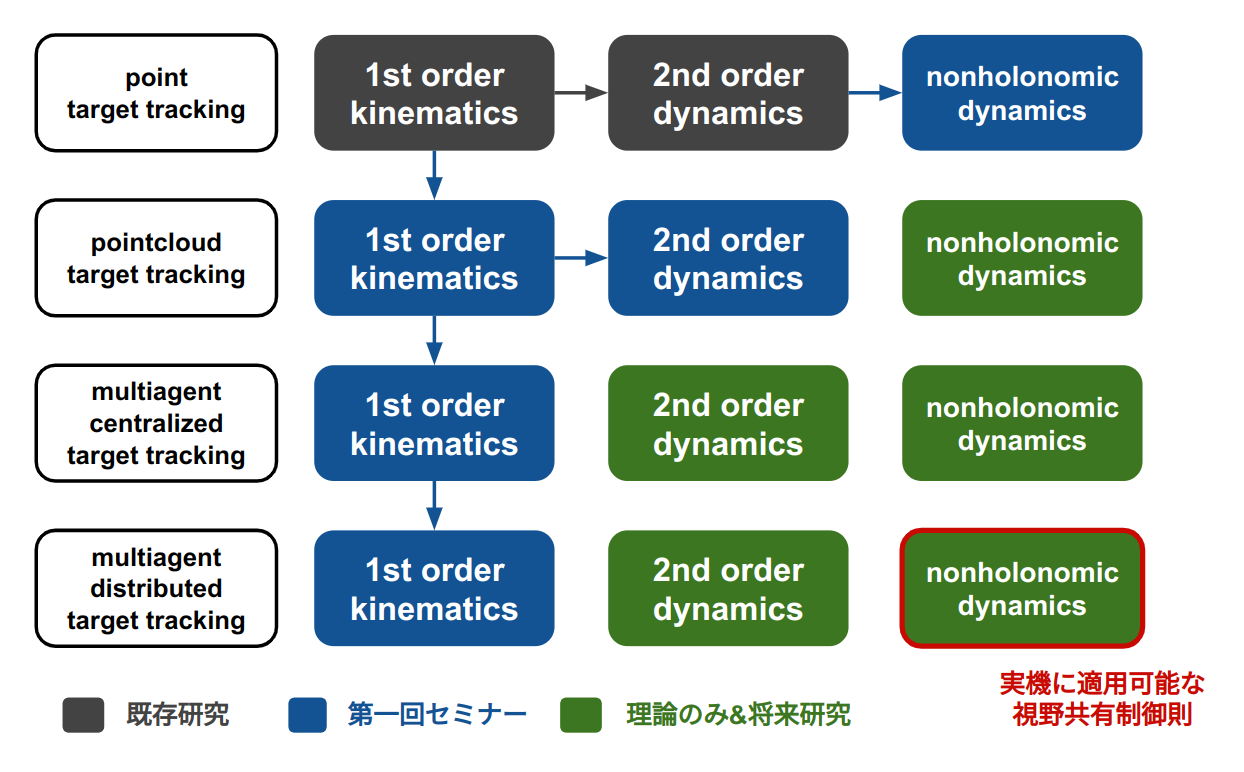
\includegraphics[width=0.8\linewidth]{fig/progress.png}
\caption{第一回セミナーの内容と本研究の貢献点}
\label{fig:progress}
\end{figure}
\section{Conclusion}

本論文では,SE(3)上における協調自己位置推定のための視野共有を保証する分散型CBFを提案した.提案手法は,単一特徴点追従,複数特徴点追従,複数エージェントの共通特徴点追従,そして二次系システムのための高次CBFへと段階的に拡張され,それぞれの場合について理論的な解析と定式化を行った.

\subsection{研究成果のまとめ}

本研究の主な成果は以下の通りである.

\begin{enumerate}
    \item SE(3)上での共有視野保証:従来研究は主に平面上の(SE(2))あるいは単眼視野の問題に限定されていたが,本研究では3次元の複雑なダイナミクス下での共有視野保証を実現した.エージェント位置を$T_i=(p_i, R_i)\in \mathrm{SE}(3)$,環境内の特徴点を$q_l\in \mathcal{L}$として,視野内条件$\beta_l^{\top}(p_i)R_ie_c-\cos\Psi_\mathcal{F}>0$に基づく安全集合を定義し,CBFを設計した.
    
    \item 特徴点に基づく確率的可視性制約とCBFの適用:各エージェントが観測する特徴点に基づき,その可視性を確率的に評価した上で,制御バリア関数(CBF)に組み込み,常時高い確率で共有視野が確保されるよう制御入力を設計した.特に,複数の特徴点を追従する場合に,安全集合$B_{i}=1-q-\prod_{l\in\mathcal{L}}(1-\phi_{i}^l)$を定義し,確率$q$以上で特徴点が視野内に保持されるよう制約を設計した.
    
    \item 非ホロノミックなドローンダイナミクスへの対応と分散最適化:機体の並進および回転運動を同時に考慮するSE(3)上の非ホロノミックドローンモデルに対して,高次制約も扱える制御バリア関数(HOCBF)を導入し,各エージェントが局所的な情報交換を通じて分散最適化アルゴリズム(PDMM)により制御解を求める枠組みを提案した.これにより,リアルタイム性とスケーラビリティの両立を実現した.
    
    \item 二次系システムのための高次CBF:実機への適用を考慮し,ドローンの二次系ダイナミクスに対応するHOCBFを設計した.SE(3)における離散ダイナミクスを導出し,ホロノミック系と非ホロノミック系それぞれに対するQP定式化を行った.これにより,より実際的なドローンモデルに対しても視野共有保証が可能となった.
\end{enumerate}

シミュレーション結果から,提案手法は安全制約を満たしながら目標位置への追従が可能であることが示された.特に,確率的アプローチにより複数の特徴点を視野内に保持する制約を滑らかに表現でき,分散実装により計算効率とスケーラビリティが向上することが確認された.また,HOCBFは二次系システムに対して滑らかな制御入力を生成し,安全制約の満足度も高いことが示された.

\subsection{今後の課題}

本研究の今後の課題として,以下の点が挙げられる.

\begin{enumerate}
    \item 実機実験による検証:本研究ではシミュレーションによる検証を行ったが,実機実験による検証は今後の課題である.特に,センサノイズや通信遅延などの実環境での不確実性に対するロバスト性の評価が必要である.
    
    \item 自己位置推定との統合:本研究では視野共有を保証するCBFを設計したが,実際の自己位置推定アルゴリズム(CoVINSなど)との統合は今後の課題である.視野共有保証と自己位置推定の精度向上の関係を定量的に評価することが重要である.
    
    \item 障害物回避との統合:実環境では障害物が存在するため,視野共有保証と障害物回避を同時に満たす制御則の設計が必要である.複数の安全制約を統合するための手法の開発が課題となる.
    
    \item スケーラビリティの向上:より多数のエージェントに対応するため,分散アルゴリズムのさらなる効率化や,グラフ構造を考慮した通信トポロジの最適化が課題である.
    
    \item 動的環境への対応:本研究では静的な環境を仮定したが,動的な環境(移動する特徴点や障害物)に対応するための拡張が必要である.特に,予測に基づく制御や適応的なCBF設計が課題となる.
\end{enumerate}

これらの課題に取り組むことで,より実用的な視野共有保証手法の開発が期待される.特に,自己位置推定との統合により,マルチロボットシステムの協調自己位置推定の精度向上に貢献できると考えられる.

本研究の成果は,ドローンの協調自己位置推定だけでなく,監視・捜索・協調輸送などの様々なマルチロボットタスクにおいて,視野共有を保証するための基盤技術として応用可能である.今後は,より複雑な環境や多様なタスクに対応するための拡張を進めていく予定である.

\begin{thebibliography}{99}
\bibitem{Sample2025} 著者名, ``論文タイトル,'' {\it ジャーナル名}, Vol. 1, No. 1, pp. 1-10, 2025.

\bibitem{LaTeX2025} LaTeX Project Team, ``LaTeX: A Document Preparation System,'' {\it Technical Report}, 2025.

\bibitem{Science2025} 科学太郎, 技術花子, ``科学技術論文の書き方,'' {\it 科学技術ジャーナル}, Vol. 10, No. 5, pp. 123-145, 2025.
\end{thebibliography}


\end{document}
